\documentclass[b5paper,openany]{standalone}
\usepackage{luatexja-preset}
\usepackage{tikz}
\usetikzlibrary{calc}

\begin{document}
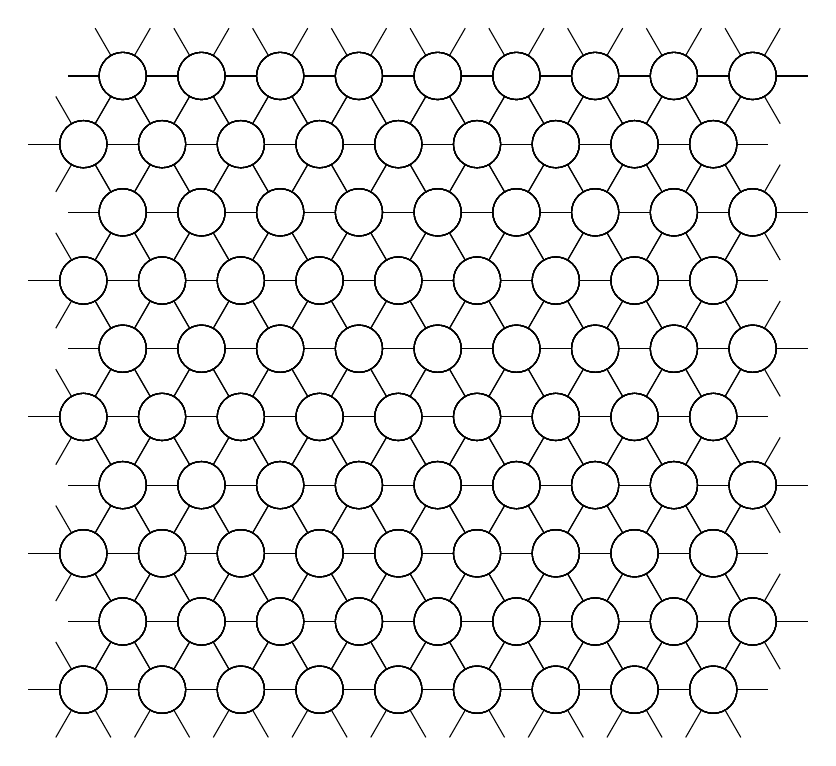
\begin{tikzpicture} % tikzpicture環境開始
\foreach \b in%
{%
	-4,-2,0,2,4%
}{%
	\foreach \a in%
	{%
		-4,-3,-2,-1,0,1,2,3,4%
	}{%
		\foreach \angle in%
		{%
			0,60,120,180,240,300%
		}{%
			\path (\a cm,\b *0.866025cm) +(\angle:0.3cm) [draw]-- +(\angle:0.7cm);
			\path (\a cm,\b *0.866025cm) ++(60:1cm) +(\angle:0.3cm)[draw] -- +(\angle:0.7cm);
			\draw (\a cm,\b *0.866025cm) circle [radius=0.3cm];
			\draw (\a cm,\b *0.866025cm) ++(60:1cm) circle [radius=0.3cm];
		}%
	}%
}%
\end{tikzpicture} % tikzpicture環境終了
\end{document}
